\Chapter{Koncepció}

\Section{A fejezet célja}

Ez a fejezet még nem a saját eredményekkel foglalkozik, hanem bemutatja, mi a problémakör, milyen módszerekkel, milyeneredményeket sikerült elérni eddig másoknak.

A hivatkozások jelentős része ehhez a fejezethez szokott kötődni.
(Egy hivatkozás például így néz ki \cite{coombs1987markup}.)
Itt lehet bemutatni a hasonló alkalmazásokat.

\Section{Tartalom és felépítés}

A fejezet tartalma témától függően változhat. Az alábbiakat attól függően különböző arányban tartalmazhatják.
\begin{itemize}
\item Irodalomkutatás. Amennyiben a dolgozat egy módszer kidolgozására, kifejlesztésére irányul, akkor itt lehet részletesen végignézni (módszertani vagy időrendi bontásban), hogy az eddigiekben milyen eredmények születtek a témakörben.
\item Technológia. Mivel jellemzően kutatásról vagy szoftverfejlesztésről van szó, ezért annak a jellemző elemeit, technikai részleteit itt kell bemutatni.
Ez tehát egy módszeres bevezetés ahhoz, hogy ha valaki nem jártas a témakörben, akkor tudja, hogy a dolgozat milyen aktuálisan elérhető eredményeket, eszközöket használt fel.
\item Piackutatás. Bizonyos témáknál új termék vagy szolgáltatás kifejlesztése a cél.
Ekkor érdemes annak alaposan utánanézni, hogy aktuálisan milyen eszközök érhetők el a piacon.
Ez szoftverek esetében a hasonló alkalmazások bemutatását, táblázatos formában történő összehasonlítását jelentheti.
Szerepelhetnek képek és észrevételek a viszonyításként bemutatott alkalmazásokhoz.
\item Követelmény specifikáció. Külön szakaszban érdemes részletesen kitérni az elkészítendő alkalmazással kapcsolatos követelményekre.
Ehhez tartozhatnak forgatókönyvek (\textit{scenario}-k).
A szemléletesség kedvéért lehet hozzájuk képernyőkép vázlatokat is készíteni, vagy a használati eseteket más módon szemléltetni.
\end{itemize}

\Section{Amit csak említés szintjén érdemes szerepeltetni}

Az olvasóról annyit feltételezhetünk, hogy programozásban valamilyen szinten járatos, és a matematikai alapfogalmakkal sem ebben a dolgozatban kell megismertetni.
A speciális eszközök, programozási nyelvek, matematikai módszerekk és jelölések persze jó, hogy ha említésre kerülnek, de nem kell nagyon belemenni a közismertnek tekinthető dolgokba.

\Section{Hasonló tervező alkalmazások}


		\SubSection{Sweet Home 3D}
		\begin{figure}[h]
			\centering
			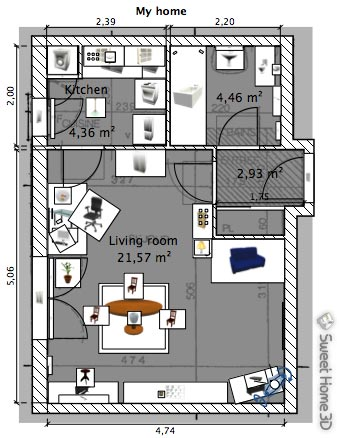
\includegraphics[scale=0.5]{images/sweethome3d_2d.jpg}
		\end{figure}
